\documentclass[12pt]{article}
\usepackage[a4paper, margin=1in]{geometry}
\usepackage{times}
\usepackage{graphicx}
\usepackage{tikz}
\usetikzlibrary{shapes.geometric, arrows.meta, positioning, calc}
\usepackage{cite}
\usepackage{setspace}
\usepackage{titlesec}
\usepackage{hyperref}

\onehalfspacing

\titleformat{\section}{\large\bfseries\scshape}{\thesection.}{1em}{}
\titleformat{\subsection}{\normalsize\bfseries}{\thesubsection.}{1em}{}

\begin{document}

\begin{center}
    {\LARGE \textbf{DefectLens: Efficient ViT-Based Anomaly Detection with Multi-Criteria Token Fusion (MCTF)} \par}
    \vspace{0.5cm}
    {\large \textbf{Ali Mohammed Maaz Mohammed Ashraf} \par}
    {\large Roll No: 2023bcs0202 \par}
    {\large Computer Vision Course Project \par}
    {\large Weekly Project Write-Up \par}
    \vspace{0.5cm}
\end{center}

\begin{abstract}
\noindent This report establishes the core motivation and structural framework for the DefectLens anomaly detection system. It delves into the computational hurdles of employing Vision Transformers (ViTs) in high-resolution manufacturing inspection. Additionally, it highlights how integrating a Multi-Criteria Token Fusion (MCTF) approach can facilitate real-time edge processing, ultimately satisfying the critical objectives of maintaining superior defect detection accuracy while drastically cutting down operational latency.
\end{abstract}

\vspace{0.5cm}

\section{Problem Statement}
In the landscape of industrial quality assurance, robust optical inspection is a cornerstone. Standard supervised machine learning paradigms are insufficient here because they depend on exhaustive datasets for every conceivable type of defect. Given that manufacturing flaws are typically scarce and highly variable, such exhaustive labeling is impossible. Therefore, the industry relies on unsupervised anomaly detection, wherein a model learns exclusively from normal, defect-free samples.

Recently, Vision Transformers (ViTs) have set new benchmarks in this domain by efficiently capturing global spatial relationships and intricate patch features. However, their primary drawback is a massive computational footprint that grows quadratically as the image sequence length increases. For industrial applications requiring high-throughput (low latency) processing of high-resolution images, the standard ViT's uniform token processing mechanism acts as a severe roadblock.

The central problem driving this research is: \textit{How can the enormous computational load of Vision Transformers be minimized for anomaly detection tasks without losing the high-resolution, pixel-level details necessary to accurately localize microscopic defects?}

\section{Motivation and Industrial Application}
A failure to catch minute manufacturing defects can cascade into catastrophic product failures, extensive recalls, and safety hazards, particularly in high-stakes fields like aerospace and medical device production. Conversely, a sluggish inspection algorithm creates a massive bottleneck on the factory floor, directly impacting yield and profitability. Successfully navigating this latency-accuracy trade-off is a paramount challenge for the future of Industry 4.0.

The motivation behind DefectLens is rooted in these demanding factory-floor dynamics, which necessitate inspection systems that are both highly precise and extraordinarily fast. While traditional Convolutional Neural Networks (CNNs) lack the global context needed for complex textures, baseline ViTs simply cannot meet the real-time processing constraints of edge hardware.

\textbf{Intended Application:} DefectLens is engineered for direct integration into Automated Optical Inspection (AOI) setups on production lines. By employing this streamlined anomaly detection framework, manufacturers can seamlessly identify structural irregularities, surface defects, and assembly discrepancies (akin to those in the MVTec AD dataset) in real-time as products pass through high-speed manufacturing pipelines.

\section{Project Objectives}
The overarching objective of the DefectLens initiative is to design and deploy an optimized industrial anomaly detection architecture that capitalizes on the deep feature extraction capabilities of Vision Transformers while systematically bypassing their computational inefficiencies. The specific goals are:

\begin{itemize}
    \item \textbf{Establishment of a Baseline:} Deploy a Vision Transformer integrated with a PatchCore-style Memory Bank to provide a resilient foundation for unsupervised anomaly detection tasks.
    \item \textbf{Token Fusion Implementation:} Embed a Multi-Criteria Token Fusion (MCTF) module that actively identifies and merges redundant, non-informative background tokens across the layers of the network, guided by the strategies outlined by Lee et al. \cite{lee2023multi}.
    \item \textbf{Information Preservation:} Utilize stringent criteria---encompassing token similarity, one-step-ahead attention, and token size limits---to ensure that the fine-grained visual details of small anomalies are rigorously protected.
    \item \textbf{Latency Optimization:} Markedly reduce the overall Floating Point Operations (FLOPs) and inference latency by decreasing the number of active tokens, making real-time edge processing viable.
    \item \textbf{Comprehensive System Development:} Package the refined model into a full-stack application featuring a FastAPI backend and a React-based frontend to emulate a real-world, interactive quality control dashboard.
\end{itemize}

\section{System Architecture Diagram}
To maintain accuracy while reducing token count, the MCTF module is seamlessly integrated between the successive blocks of the Vision Transformer. Figure \ref{fig:architecture} demonstrates the end-to-end workflow, beginning with image acquisition and concluding with the generation of an anomaly heatmap.

\begin{figure}[htpb]
    \centering
    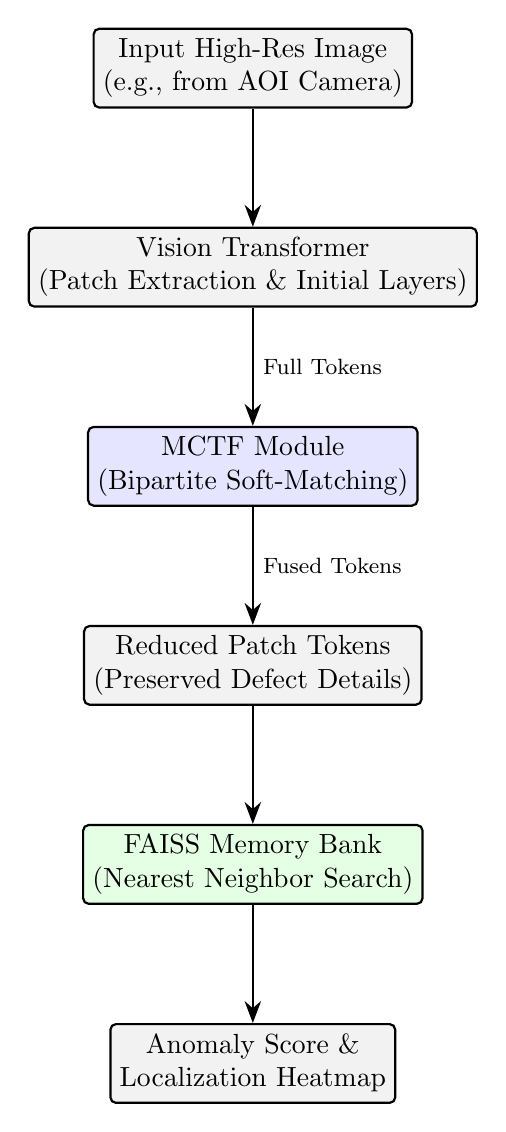
\begin{tikzpicture}[
        node distance=1.5cm and 1cm,
        box/.style={rectangle, draw=black, thick, minimum width=3.5cm, minimum height=1cm, align=center, fill=gray!10, rounded corners=2pt},
        arrow/.style={-{Stealth[scale=1.2]}, thick}
    ]
        % Nodes
        \node[box] (input) {Input High-Res Image \\ (e.g., from AOI Camera)};
        \node[box, below=of input] (vit) {Vision Transformer \\ (Patch Extraction \& Initial Layers)};
        \node[box, below=of vit, fill=blue!10] (mctf) {MCTF Module \\ (Bipartite Soft-Matching)};
        \node[box, below=of mctf] (fused) {Reduced Patch Tokens \\ (Preserved Defect Details)};
        \node[box, below=of fused, fill=green!10] (memory) {FAISS Memory Bank \\ (Nearest Neighbor Search)};
        \node[box, below=of memory] (output) {Anomaly Score \& \\ Localization Heatmap};

        % Arrows
        \draw[arrow] (input) -- (vit);
        \draw[arrow] (vit) -- node[right, font=\footnotesize] {Full Tokens} (mctf);
        \draw[arrow] (mctf) -- node[right, font=\footnotesize] {Fused Tokens} (fused);
        \draw[arrow] (fused) -- (memory);
        \draw[arrow] (memory) -- (output);
    \end{tikzpicture}
    \caption{High-Level Architecture of DefectLens integrating MCTF.}
    \label{fig:architecture}
\end{figure}

\section{Core Ideas and References}
The architecture and methodology of this project are significantly influenced by leading research in Vision Transformer optimization. Specifically, the token reduction framework draws heavily on the pioneering work of Lee et al. \cite{lee2023multi}. Their proposed use of ``one-step-ahead attention'' serves as a critical evaluative mechanism, enabling the network to proactively preserve tokens that are slated to receive high attention in subsequent layers. This mechanism is paramount for ensuring that microscopic defect signatures are not lost during the fusion process.

\begin{thebibliography}{9}
\bibitem{lee2023multi}
Sanghyeok Lee, Joonmyung Choi, and Hyunwoo J. Kim,
\textit{``Multi-criteria Token Fusion with One-step-ahead Attention for Efficient Vision Transformers,''}
Department of Computer Science and Engineering, Korea University.
Emails: \{cat0626, pizard, hyunwoojkim\}@korea.ac.kr.
\end{thebibliography}

\end{document}
